\documentclass[12pt]{article}
\usepackage{graphicx}
\usepackage{wrapfig}
\openup 1em

\title{Security Vulnerabilities in the Veterinary Science Building}
\date{2017-05-09}
\author{Richard Coleman\
        \and
        Nora Cook
        \and
        Nakhai Bradley Johnson
        }
\begin{document}
        \maketitle
        \newpage
\section{Introduction}
        The Alfred State veterinary science building is a few miles away from the 
        Alfred State College and is used by students in the veterinary field. The
        building is closed completely on weekends. On weekdays it is open and while
        normally there are students there, during finals week it is almost empty.

\section{Security}
        \subsection{Vulnerabilities}
        
        \begin{wrapfigure}{R}{0.3\textwidth}
        \centering
        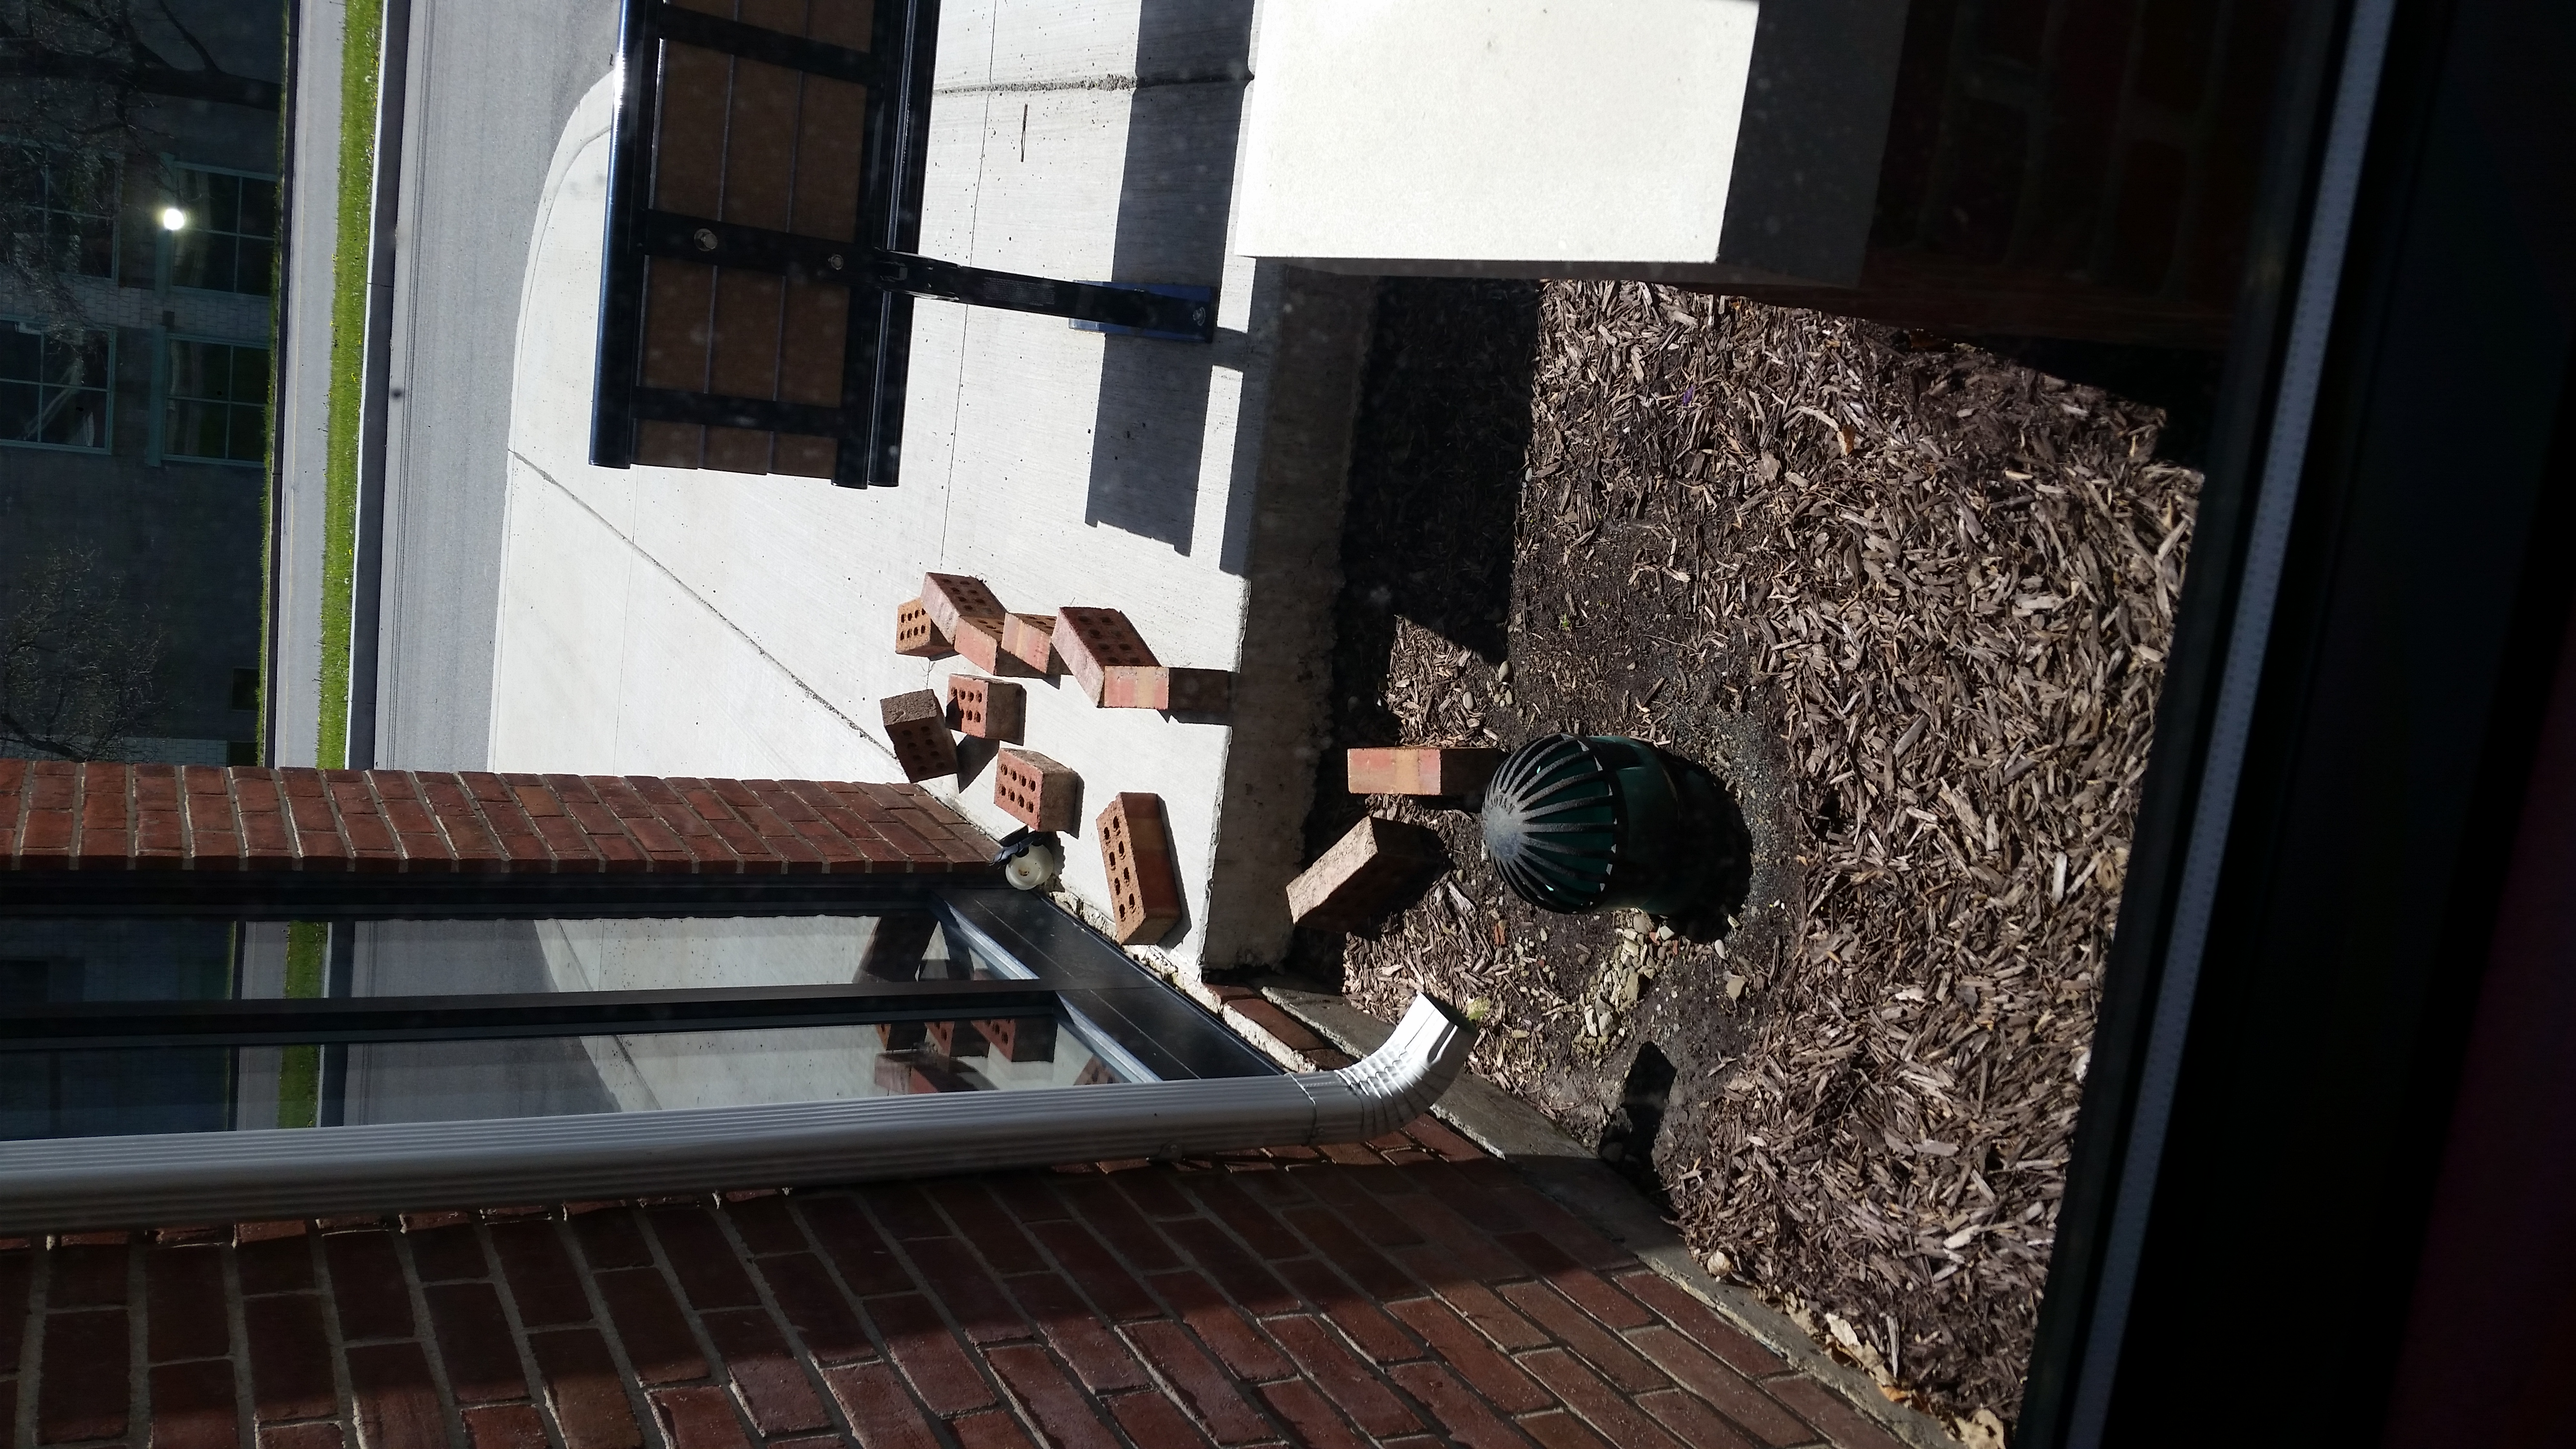
\includegraphics[width=0.5\textwidth, height=0.25\textwidth, angle=270]{img/bricks.jpg}
        \end{wrapfigure}

        When approaching the building from the main entrance you can see a pile of 
        bricks laying right beside the door. Someone that is very intent on breaking
        into the building could simply use any of those bricks to break any of the 
        large glass windows around the building.
        
        \begin{wrapfigure}{R}{0.3\textwidth}
        \centering
        \includegraphics[width=0.5\textwidth, height=0.25\textwidth, angle=270]{img/camera.jpg}
        \end{wrapfigure}

        After entering the building you can see only one security camera, our team
        did not find any more. There is also a secretary desk with a completely 
        unlocked computer. There are also two snakes in easily movable terrariums.

\end{document}
